\documentclass[Master,Submit,UKenglish]{scrbook}
%------------------------------------------------------------------------------
% This file contains a skeleton thesis for
% a Physics or Astronomy Institute in the University of Bonn

% Specify the thesis type as an option: PhD, Master, Diplom, Bachelor
% Specify the thesis stage as an option: Draft (default), Submit, Final, PILibrary

% Specify the language(s) in the class and then use babel.
% If you need more than one language, give the default language last,
% e.g. ngerman,UKenglish for a thesis in British (UK) English where you want
% to be able to set the language to German for some part of it.

%------------------------------------------------------------------------------
% Pass TeX Live version to the package
% Use command pdflatex --version to find out which version you are running
% Add option backref=false when your thesis is ready to turn off back-referencing
% in your bibliography
\usepackage[texlive=2016]{ubonn-thesis}
% Adjustments to standard biblatex style
\usepackage[showurl=false]{ubonn-biblatex}

\usepackage{epigraph}

\numberwithin{equation}{chapter}

% Glossary package
% \usepackage[acronym,toc,nosuper]{glossaries}
% TikZ packages and libraries
\usepackage{tikz}
% \usepackage{tikz-3dplot}
% \usetikzlibrary{positioning,shapes,arrows}
\usetikzlibrary{decorations.pathmorphing}
\usetikzlibrary{calc}
% \usetikzlibrary{decorations.markings}

\usepackage{pgfplots}
\usepgfplotslibrary{fillbetween}

\usepackage{thesis_defs}

% user-defined packages and definitions
% Fonts and languages

% Multilingual support
%\usepackage{polyglossia}

% more symbols
\usepackage{textcomp}

% AMS--related
\usepackage{amsmath,amssymb}

% ':=' as \coloneqq
\usepackage{mathtools}
% Physical bras and kets
\usepackage{braket}
% SI units
\usepackage{siunitx}
\sisetup{separate-uncertainty}

\usepackage{graphicx}
%\usepackage[colorinlistoftodos]{todonotes}


% Boxed equations. NEED TO BE LOADED BEFORE unicode-math!
\usepackage{empheq}
% Theorems
\usepackage{amsthm}

% Chemical elements
%\usepackage[version=4]{mhchem}


%\usepackage{fancybox}

\usepackage{enumitem} % \begin{enumerate}[label=\Alph*]


% Other formats

% Labelling equations according to sections
\numberwithin{equation}{section}


% Bibliography in the main text!!!

%\usepackage[
			%style=alphabetic,
%			backend=biber]{biblatex}
%\usepackage{hyperref}
\usepackage{nameref}

% Cross-references
% The \newtheorem commands have to come after the loading of {cleveref}.
% Additionally, the cleverref package has to be loaded after ntheorem or
% amsthm. cleverref has to be loaded after hyperref!
\usepackage{cleveref}
%\usepackage{nameref}%,thmtools}

% Plot
\usepackage{tikz}
\usetikzlibrary{decorations.pathmorphing}
\usetikzlibrary{calc}
% save compiled tikz plots; enable --shell-escape
%\usetikzlibrary{external}
%\tikzexternalize[prefix=./tikz/]

% Fontspec fot XeLaTeX
\usepackage{fontspec}
	% Unicode fonts
	\setmainfont{CMU Serif}
	\setsansfont{CMU Sans Serif}
	\setmonofont{CMU Typewriter Text}
	% declare a command \doulos to load the Doulos SIL font
	%\newfontfamily\brill{Brill}
	% now create a \textIPA{} command
	%\DeclareTextFontCommand{\textIPA}{\brill}
\usepackage{amsfonts}
\usepackage{unicode-math}
\usepackage{unicode-math}
	\setmathfont{Latin Modern Math} % default
	%\setmathfont[range=\mathalpha]{Asana Math}
	\setmathfont{Asana Math}[range={\mathbin}] %\mathord
	\setmathfont{STIX Math}[range={"02609}] % ☉
	\setmathfont{XITS Math}[range={"1D4B6-"1D4CF}] % Script, Latin, lowercase
	\setmathfont{Latin Modern Math}[range={"1D608-"1D63B}, sans-style=italic]
	\setmathfont{Latin Modern Math}[range={
		"00391-"003A9,
		"003B1-"003F5, 
		"1D6A8-"1D6E1},	% Bold Greek
		sans-style=upright]
	%\setmathfont{⟨font name⟩}[range=⟨unicode range⟩,⟨font features⟩]

% Math symbols and user-defined extensions


% some unicode characters
% ≙ for equal with hat


% Mathematical constants
\newcommand{\ii}{{\Bbbi}}
\newcommand{\ee}{{\Bbbe}}
\newcommand{\pp}{{\Bbbpi}}

% Bracket-like
\newcommand{\rbr}[1]{{\left(#1\right)}}
\newcommand{\sbr}[1]{{\left[#1\right]}}
\newcommand{\cbr}[1]{{\left\{#1\right\}}}
\newcommand{\abr}[1]{{\left<#1\right>}}
\newcommand{\vbr}[1]{{\left|#1\right|}}
\newcommand{\dvbr}[1]{{\left\|#1\right\|}}
\newcommand{\fat}[2]{{\left.#1\right|_{#2}}}
% Functions; note the space between the name and the bracket!
\newcommand{\rfun}[2]{{#1}\mathopen{}\left(#2\right)\mathclose{}}
\newcommand{\sfun}[2]{{#1}\mathopen{}\left[#2\right]\mathclose{}}
\newcommand{\cfun}[2]{{#1}\mathopen{}\left\{#2\right\}\mathclose{}}
\newcommand{\afun}[2]{{#1}\mathopen{}\left<#2\right>\mathclose{}}
\newcommand{\vfun}[2]{{#1}\mathopen{}\left|#2\right|\mathclose{}}
% Differentials
\newcommand{\DD}{\BbbD}
\newcommand{\dd}{\Bbbd}
\newcommand{\dva}{\mupdelta} % no better way?!
% Fraction-like
\newcommand{\frde}[2]{{\frac{\dd{#1}}{\dd{#2}}}}
\newcommand{\frDe}[2]{{\frac{\DD{#1}}{\DD{#2}}}}
\newcommand{\frpa}[2]{{\frac{\partial{#1}}{\partial{#2}}}}
\newcommand{\frdva}[2]{{\frac{\dva{#1}}{\dva{#2}}}}
% Equal marks
\newcommand{\eeq}{{\overset{!}{=}}}
\newcommand{\lls}{{\overset{!}{<}}}
\newcommand{\ggt}{{\overset{!}{>}}}
\newcommand{\lle}{{\overset{!}{\le}}}
\newcommand{\gge}{{\overset{!}{\ge}}}
% overline-like marks
\newcommand{\ol}[1]{{\overline{{#1}}}}
\newcommand{\ul}[1]{{\underline{{#1}}}}
\newcommand{\tld}[1]{{\widetilde{{#1}}}}
\newcommand{\ora}[1]{{\overrightarrow{#1}}}
\newcommand{\ola}[1]{{\overleftarrow{#1}}}
\newcommand{\td}[1]{{\widetilde{#1}}}
\newcommand{\what}[1]{{\widehat{#1}}}
%\newcommand{\prm}{{\symbol{"2032}}}

% Math operators
% Why does \DeclareMathOperator not work?
\DeclareMathOperator{\sgn}{sgn}
\DeclareMathOperator{\grad}{grad}
\DeclareMathOperator{\curl}{curl}
\DeclareMathOperator{\rot}{rot}
\DeclareMathOperator{\opdiv}{div}
\DeclareMathOperator{\opdeg}{deg}

\DeclareMathOperator{\sech}{sech}
\DeclareMathOperator{\csch}{csch}

\DeclareMathOperator{\diag}{diag}
\DeclareMathOperator{\tr}{tr}

\DeclareMathOperator{\ad}{ad}

\DeclareMathOperator{\expi}{expi}

% Group and Algebras
\newcommand{\SO}{\mathsf{SO}\,}
\newcommand{\SU}{\mathsf{SU}\,}
\newcommand{\so}{\mathfrak{so}\,}
\newcommand{\su}{\mathfrak{su}\,}


% amsthm
\newcommand{\thistheoremname}{} % for generic stuff
% definition of new styles
\newtheoremstyle{varplain}% name
	{}{}%      Spaces above and below, empty = `usual value'
	{\itshape}% Body font
	{}%         Indent amount (empty = no indent, \parindent = para indent)
	{\bfseries}% Thm head font
	{}%        Punctuation after thm head
	{\newline}% Space after thm head: \newline = linebreak
	{{\normalfont\thmnumber{(#2)}}\thmname{ #1}{\normalfont\thmnote{ (#3)}}}
	%         Thm head spec
\newtheoremstyle{vardefinition}% name
	{}{}%      Spaces above and below, empty = `usual value'
	{\upshape}% Body font
	{}%         Indent amount (empty = no indent, \parindent = para indent)
	{\bfseries}% Def head font
	{}%        Punctuation after thm head
	{\newline}% Space after thm head: \newline = linebreak
	{{\normalfont\thmnumber{(#2)}}\thmname{ #1}{\normalfont\thmnote{ (#3)}}}
	%         Thm head spec
\newtheoremstyle{varremark}% name
	{}{}%      Spaces above and below, empty = `usual value'
	{\upshape}% Body font
	{}%         Indent amount (empty = no indent, \parindent = para indent)
	{\itshape}% Rem head font
	{}%        Punctuation after thm head
	{\newline}% Space after thm head: \newline = linebreak
	{{\normalfont\upshape\thmnumber{(#2)}}\thmname{ #1}{\normalfont\thmnote{ (#3)}}}
	%         Thm head spec
% Plain style
\theoremstyle{plain}% default
\newtheorem{thm}{Theorem}[section]
\newtheorem{lem}[thm]{Lemma}
\newtheorem{prop}[thm]{Proposition}
% Definition style
\theoremstyle{definition}
\newtheorem{defn}{Definition}[section]
\newtheorem{exmp}{Example}[section]
\newtheorem{ppty}{Property}[section]
% Remark style
\theoremstyle{remark}
\newtheorem*{rem}{Remark}
% variant plain style
\theoremstyle{varplain}
% for specifying a named theorem with numbering
\newtheorem{genericthm}{\thistheoremname}[section]
\newenvironment{namedthm}[1]
	{\renewcommand{\thistheoremname}{#1}%
		\begin{genericthm}}
	{\end{genericthm}}
% for specifying a named theorem without numbering
\newtheorem*{genericthm*}{\thistheoremname}
\newenvironment{namedthm*}[1]
	{\renewcommand{\thistheoremname}{#1}%
		\begin{genericthm*}}
	{\end{genericthm*}}
\newtheorem{unamedthm}[genericthm]{Theorem}
% variant definition style
\theoremstyle{vardefinition}
% for specifying a named definition with numbering
\newtheorem{genericdef}[genericthm]{\thistheoremname}
\newenvironment{nameddef}[1]
	{\renewcommand{\thistheoremname}{#1}%
		\begin{genericdef}}
	{\end{genericdef}}
% for specifying a named definition without numbering
\newtheorem*{genericdef*}{\thistheoremname}
\newenvironment{nameddef*}[1]
	{\renewcommand{\thistheoremname}{#1}%
		\begin{genericdef*}}
	{\end{genericdef*}}
\newtheorem{unameddef}[genericthm]{Definition}
% variant remark style
\theoremstyle{varremark}
% for specifying a named  with numbering
\newtheorem{genericrem}[genericthm]{\thistheoremname}
\newenvironment{namedrem}[1]
	{\renewcommand{\thistheoremname}{#1}%
		\begin{genericrem}}
	{\end{genericrem}}
% for specifying a name without numbering
\newtheorem*{genericrem*}{\thistheoremname}
\newenvironment{namedrem*}[1]
	{\renewcommand{\thistheoremname}{#1}%
		\begin{genericrem*}}
	{\end{genericrem*}}
\newtheorem{unamedrem}[genericthm]{Remark}


% cleveref
\crefname{lem}{lemma}{lemmas}
\Crefname{lem}{Lemma}{Lemmas}
\crefname{thm}{theorem}{theorems}
\Crefname{thm}{Theorem}{Theorems}
\crefname{defn}{definition}{definitions}
\Crefname{defn}{Definition}{Definitions}
\crefname{exmp}{example}{examples}
\Crefname{exmp}{Example}{Examples}
\crefname{namedthm}{}{}
\Crefname{namedthm}{}{}
% Physical constants
\newcommand{\lc}{\mitsansc} % speed of light
\newcommand{\bk}{\mitsansk} % Boltzmann's constant
\newcommand{\phs}{\hslash} % reduced Planck constant
\newcommand{\ph}{\Planckconst} % Planck constant
\newcommand{\hH}{\mitsansH} % Hubble constant H
\newcommand{\hh}{\mitsansh} % Hubble constant h

\newcommand{\plm}{m_\text{P}} % Planck mass
\newcommand{\pll}{l_\text{P}} % Planck length
\newcommand{\plt}{t_\text{P}} % Planck time

\newcommand{\nG}{\mitsansG} % Newton's constant
\newcommand{\aN}{\mitsansN} % Avogadro number
\newcommand{\ec}{\mitsanse} % unit electric charge

\newcommand{\gR}{\mitsansR} % gas constant

\newcommand{\apE}{\alpha_\text{E}} % EM fine struct const
\newcommand{\apG}{\alpha_\text{G}} % Grav fine struct const

% Common symbols
\newcommand{\Ld}{\mscrL} % Lagrangian density
\newcommand{\fp}{p_\text{F}} % Fermi momentum
\newcommand{\fE}{\mscrE_\text{F}} % Fermi energy

% Others
\newcommand{\rSch}{R_\text{S}} % Schwarzschild radius

\newcommand{\fHor}{{h^+}} % future horizon
\newcommand{\pHor}{{h^-}} % past horizon

% siunitx
% Astronomy
\DeclareSIUnit\parsec{pc}
\DeclareSIUnit\lightyear{ly}

%------------------------------------------------------------------------------
% Instead of colouring  links, cites, table of contents etc.
% put them in a coloured box for the screen version.
% This is probably a good idea when you print your thesis.
% \hypersetup{colorlinks=false,
%   linkbordercolor=blue,citebordercolor=magenta,urlbordercolor=darkgreen
% }

%------------------------------------------------------------------------------
% When writing your thesis it is often helpful to have the date and
% time in the output file. Comment this out for the final version.
\ifoot[\today{} \thistime]{\today{} \thistime}

% In order to check if your labels are referenced try the refcheck package
% \usepackage{refcheck}

%------------------------------------------------------------------------------
% biblatex is included by ubonn-thesis. Look there for the settings used.
% See the options for settings that can be changed easily.
% For further changes copy the \RequirePackage[...]{biblatex} here
% and include ubonn-thesis with the option biblatex=false.

% Specify the bibliography files here and not at the end!
% Use standard_refs-bibtex if you use bibtex or bibtex8
% and standard_refs-biber  if you use biber
\addbibresource{thesis_refs.bib}
\addbibresource{../refs/standard_refs-biber.bib}

%------------------------------------------------------------------------------
% The following definitions are used to produce the title pages
% needed at various stages
\newcommand{\thesistitle}{Hawking Radiation: A Comparison of Pure-state and 
Thermal Descriptions}
\newcommand*{\thesisauthor}{王\ 一帆 Yi-Fan Wang }
\newcommand*{\thesistown}{四川 Sichuan}
\renewcommand*{\InstituteName}{\ITPK}
\renewcommand*{\inInstitute}{\inITPK}
\renewcommand*{\InstituteAddress}{\ITPKaddress}
% Adjust \thesisreferee...text depending on male/female referee
\newcommand*{\thesisrefereetwotext}{1.\ Gutachter}
\newcommand*{\thesisrefereetwo}{Prof.\ Dr.\ Claus Kiefer}
\newcommand*{\thesisrefereeonetext}{2.\ Gutachter}
\newcommand*{\thesisrefereeone}{Prof.\ Dr.\ Hans-Peter Nilles}
% Date when thesis was submitted (Master/Diplom)
% Year or Month, Year when thesis was submitted (PhD)
\newcommand*{\thesissubmit}{13.02.2017}
% \newcommand*{\thesissubmit}{Month 2016}
% Date of thesis examination (PhD)
\newcommand*{\thesispromotion}{10.02.2017}
% Month and year of the final printed version of the thesis
\newcommand*{\thesismonth}{February}
\newcommand*{\thesisyear}{2017}
\newcommand*{\thesisnumber}{BONN-IR-2017-XXX}

%------------------------------------------------------------------------------
% The abstract is only needed for the printed version and should be in
% English regardless of the language of the thesis
\newcommand{\thesisabstract}{%
  \begin{otherlanguage}{UKenglish}
    %This is your thesis abstract. It may be in a language that is
    %different from the rest of your thesis.
The cases of the Hawking radiation field being described by a pure state and by 
the usual thermal state are compared within the CGHS dilaton gravity model. The 
field-strength fluctuations of the Fourier modes are computed, showing a 
discrepancy in the low-energy regime, while coinciding at high energies. Then by 
defining a distance for density operators and evaluating it for the cases 
concerned, the difference between the pure and thermal descriptions is 
quantified and found to be exponentially small with respect to the Hawking 
temperature. Possible physical interpretations are discussed.
  \end{otherlanguage}
}

%------------------------------------------------------------------------------
% \includeonly can be used to select which chapters you want to process
% A simple \include command just inserts a \clearpage before and after the file
% Note that \includeonly can be quite picky! Do not forget to put a
% comma after the filename, otherwise it will simply be ignored!
% \includeonly{%
%   thesis_intro,
%   thesis_appendix,
%   thesis_acknowledge
% }

%------------------------------------------------------------------------------
% Give a list of directories where figures can be found. Do not leave
% any spaces in the list and end the directory name with a /
\graphicspath{%
  {../figs/}%
  {../figs/cover/}%
  {../figs/graphics/}%
  {../feynmf/}%
}

%------------------------------------------------------------------------------
% Make a glossary and a list of acronyms
% \makeglossaries

% Glossary entries
% \input{thesis_glossary}

% Draft version - add the word DRAFT on the cover pages
\ifthenelse{\equal{\ThesisVersion}{Draft}}{%
  \usepackage{background}
  \ifthenelse{\texlive < 2013}{%
    \SetBgContents{DRAFT}
    \SetBgColor{blue!30}
  }{%
    \backgroundsetup{contents=DRAFT, color=blue!30}
  }
}

%------------------------------------------------------------------------------
\begin{document}

% Cover page of thesis - this is only needed for the printed final
% version to be submitted to the department library
% Do not use this page for thesis submission to the Prüfungsamt or Promotionsbüro!
\ifthenelse{\equal{\ThesisVersion}{PILibrary}}{%
  \typeout{Document \jobname, Info: PI library version of thesis}
  \input{../cover/\ThesisType_Cover}
}{}

% Start counting pages from the title page
\frontmatter
% Dedication has to come before \maketitle
% \dedication{For ...}

% Select the correct title page(s)
\ifthenelse{\equal{\ThesisType}{Unknown}}{%
  \typeout{Document \jobname, Error: Unknown thesis type - no title page printed}
}{%
  % Bachelor thesis only has one title page
  \ifthenelse{\equal{\ThesisType}{Bachelor}}{%
    \typeout{Document \jobname, Info: Bachelor thesis}
    \input{../cover/\ThesisType_Title}
  }{%
    \ifthenelse{\equal{\ThesisVersion}{Final} \OR \equal{\ThesisVersion}{PILibrary}}{%
      % Final and PI library versions
      \typeout{Document \jobname, Info: Final version of a \ThesisType  thesis}
      \input{../cover/\ThesisType_Final_Title}
    }{% Submission and draft versions
      \input{../cover/\ThesisType_Submit_Title}
      \typeout{Document \jobname, Info: Draft/submission version of a \ThesisType  thesis}
    }
  }
}

\pagestyle{scrplain}

%------------------------------------------------------------------------------
% You can add your acknowledgements here - don't forget to also add
% them to \includeonly above
%------------------------------------------------------------------------------
%\chapter*{Acknowledgements}
%\label{chap:dedi}
%------------------------------------------------------------------------------

\vspace*{\fill}
To 劉\ 青藍 (Qinglan Liu) I dedicate this thesis, for all her love and support.
\vspace*{\fill}


%You should probably use \texttt{\textbackslash chapter*} for
%acknowledgements at the beginning of a thesis and
%\texttt{\textbackslash chapter} for the end.

%%% Local Variables: 
%%% mode: latex
%%% TeX-master: "../mythesis"
%%% End: 


\tableofcontents

\mainmatter
\pagestyle{scrheadings}

% Turn off DRAFT for the following pages
\ifthenelse{\equal{\ThesisVersion}{Draft}}{%
  \ifthenelse{\texlive < 2013}{%
    \SetBgContents{}
  }{%
    \backgroundsetup{contents={}}
  }
}{}

%------------------------------------------------------------------------------
% Add your chapters here - don't forget to also add them to \includeonly above
%==============================================================================
\chapter{Introduction}
\label{sec:intro}
%==============================================================================

\epigraph{Our mistake is not that we take our theories too seriously, but that 
we do not take them seriously enough.}{Steven Weinberg 
\cite{Weinberg1993first}}

Although widely accepted, Hawking radiation remains a field of heated 
discussion and active research, especially in the interpretation and 
extrapolation of it. Being one of the first conclusions of the original 
calculation, Hawking temperature was deduced from a \emph{pure state} of the 
quantum field in the background space-time of a collapsing body, whereas a 
temperature in statistical physics is usually derived from a statistical 
ensemble in equilibrium, described by a \emph{thermal} and \emph{mixed state}. 
This discrepancy itself has since long been largely ignored, albeit related 
issues have always been in spotlight, for instance the \emph{information loss 
problem} , the \emph{origin of black hole entropy} \cite{Mann2015,Harlow2016}, 
etc. A detailed investigation of the pure and thermal descriptions would help 
understanding the aforementioned questions by laying them on a more solid 
foundation.

In this work, which is motivated by \cite{Kiefer2001,Hsu2009}, the focus is to 
reveal and quantify the difference between the two cases mentioned above. 
\Cref{chap:hawrad} is a review of Hawking radiation in the 
$\rbr{3+1}$-dimensional Einstein gravitation which is basically along 
\citeauthor{Hawking1976}'s original line, as well as that in 
$\rbr{1+1}$-dimensional dilaton gravity, also known as the  
Callan--Giddings--Harvey--Strominger (CGHS) model, in which the quantum field 
theory in curved space-time not only can be \emph{derived} from the full theory 
of quantum gravity, but also be solved exactly. Then in \cref{chap:corr_field}, 
motivated by the coincidence of the particle-number expectations, which are the 
diagonal elements of the density operators, the author computes the correlator 
of field strength, so as to reveal the difference in the off-diagonal elements. 
In \cref{chap:quantifing}, inspired by a new foundation of statistical physics, 
which is based on exact results in quantum information theory, the author 
quantifies the discrepancy between the two cases by calculating the trace 
distance between them, and the results are shown to be in accordance with the 
quantum-informational foundation, as well as those in \cref{chap:corr_field}. 
\Cref{chap:summary} is summary and outlook.

In the appendices, \cref{sec:1+1ddlt} explains more details about the CGHS 
model, \cref{chap:harosc} collects some useful results in quantised simple 
harmonic oscillator, and \cref{chap:distappd} introduces trace distance and 
fidelity.

Throughout the text, the \emph{natural units} will be used unless specified, 
where the speed of light in vacuum $\lc$, the reduced Planck constant $\phs$ and 
Boltzmann constant $\bk$ are all set to unity, while the Newton constant $\nG$ 
is kept.




%%% Local Variables: 
%%% mode: latex
%%% TeX-master: "../mythesis"
%%% End: 


%==============================================================================
\chapter{Hawking Radiation}
\label{chap:hawrad}
%==============================================================================

%------------------------------------------------------------------------------
\section{$(3+1)$-dimensional Einstein gravitation}
\label{sec:hawrad-einstein}
%------------------------------------------------------------------------------

Based on the advances in the geometry of space-time and `mechanics' of black 
holes, as well as in quantum field theory in curved space-time, 
\citeauthor{HAWKING1974} quantitatively revealed a semi-classical property of 
the black holes in \cite{HAWKING1974}. In his model, the Einsteinian 
gravitational 
background is fixed to be that of a spherically collapsing body\footnote{A 
detailed account for space-times of collapsing body can be found in 
\cite{Joshi2007}.}, the conformal diagram of which is shown in 
\cref{fig:sph-col-bod}. A neutral (real), massless scalar field $\rfun{\phi}{x}$ 
is minimally coupled to the gravitational background, so the action of the model 
reads
\begin{equation}
S \coloneqq \int_{\mscrM} {\dd^4 x} \,\sqrt{-g}\,
\cbr{g^{\mu\nu}\rbr{\partial_\mu \phi}\rbr{\partial_\nu \phi}}.
\end{equation}
One quantises the scalar field canonically on the Cauchy surface $\mscrI^-$ by 
introducing ladder operators $a^\mp$'s, and on $\mscrI^+ \cup \mscrH^+$ by 
$b^\mp$'s (for $\mscrI^+$) and $c^\mp$'s (for $\mscrH^+$). An \emph{early-time 
vacuum} is defined by
\begin{equation}
	\rfun{a^-}{p}\Ket{h} \coloneqq 0,
\end{equation}
where $\rfun{a^-}{p}$ annihilates a particle with momentum $p$, so that
\begin{equation}
\abr{\rfun{{n}_a}{p}}_h \coloneqq \Braket{h | \rfun{{n}_a}{p} | h} 
\equiv 0,\qquad \forall p,
\end{equation}
where $\rfun{n_a}{p} = \rfun{a^+}{p}\rfun{a^-}{p}$ is the number operator of 
mode with momentum $p$. This means that an asymptotic observer at early time, 
whose definition of particles agrees with $a^\mp$, detects no particle.

\begin{figure}
\begin{center}
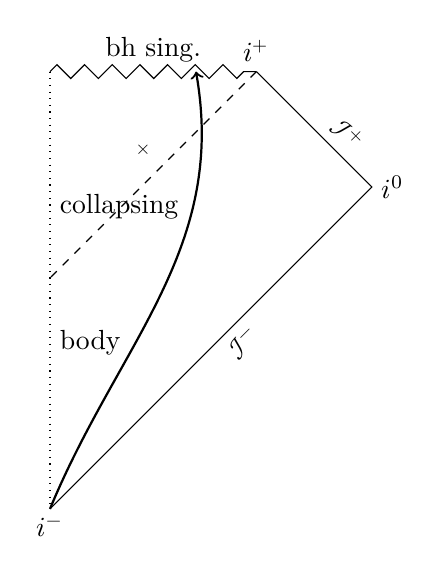
\begin{tikzpicture}%[scale=2]
\pgfmathsetmacro\myunit{3} 
\pgfmathsetmacro\sc{1.41421 35623 73095 04880 16887 24209 69807 85696 71875}
\pgfmathsetmacro\grs{0.6180339887498949}
\pgfmathsetmacro\grb{1.6180339887498949}
	\draw [decorate, decoration=zigzag] (0,0)
		-- ++ (+  0: \sc * \grs * \myunit)
			node [above] {$i^+$}
			node [pos = .5, above] {bh sing.}
			coordinate (i+);
	\draw [dotted] (0,0)
			\pgfextra{\pgfmathparse{(\grs/\sc+\sc)*\myunit}}
		-- ++ (- 90: \pgfmathresult)
			node [below] {$i^-$}
			node [pos = .31, right] {collapsing}
			node [pos = .62, right] {body}
			coordinate (i-);
	\draw (i+)
		\pgfextra{\pgfmathparse{(1 - \grs/2)*\myunit}}
		-- ++ (- 45: \pgfmathresult)
			node [right] {$i^0$}
			node [pos = .5, above right, sloped] {$\mscrI^+$}
			coordinate (i0)
		-- (i-)
			node [pos = .5, below right, sloped] {$\mscrI^-$};
	\draw [dashed] (i+)
		-- ++ (-135: 2 * \grs * \myunit)
			node [pos = .4, above left, sloped] {$\mscrh^+$};
	\draw [thick, out = 67.5, in = -80, thick, ->] (i-)
			to (\grs * \myunit, 0);
\end{tikzpicture}

\end{center}
\caption[Spherically collapsing body in Einstein gravitation]{A schematic 
conformal diagram of a spherically collapsing body in Einstein gravitation, in 
which massive matter (presumably a star) spherically collapses by gravitational 
interaction. The boundary of the collapsing body is denoted by the thick
line with arrow. The quantum field is solved on $\mscrI^-$ and $\mscrI^+ \cup 
\mscrh^+$. \label{fig:sph-col-bod}}
\end{figure}

For asymptotic observers, \citeauthor{Hawking1975} was able to evaluate the 
\emph{late-time} properties, or those with respect to the $b$'s, of 
$\Ket{h}$. He derived in \cite{Hawking1975} that\footnote{Possible divergent 
$\rfun{\delta}{0}$ factors in the particle-number expectations have been 
systematically ignored.}
\begin{equation}
\abr{\rfun{{n}_b}{\omega}}_h \approx
\Gamma_\omega\rbr{\ee^{2\pp\omega/\kappa}-1}^{-1},
\label{eq:hawking-distri}
\end{equation}
where $0 < \Gamma_\omega < 1$ is the \emph{grey-body factor}, and $\omega$ 
being the angular frequency of the mode regarded. Comparing 
\cref{eq:hawking-distri} with that of a Bose--Einstein distribution, or a 
\emph{black-body} radiation field,
\begin{equation}
\abr{\rfun{{n}}{\omega}}_\text{BE} = \rbr{\ee^{\omega/T} - 1}^{-1},
\end{equation}
it is appealing to conclude that \cref{eq:hawking-distri} describes a 
\emph{grey-body} radiation field, with the temperature
\begin{equation}
T_\text{H} \coloneqq \kappa/2\pp \equiv \phs/\lc \bk \cdot \kappa/2\pp,
\label{eq:hawking-temperature}
\end{equation}
also named after \citeauthor{Hawking1975}, and an absorption coefficient 
$\Gamma_\omega$.

\citeauthor{Hawking1975} himself argued that his calculation also holds for 
a matter field with spin, as well as for the collapse result being a rotating 
black hole. Further quantities could also be obtained in the background of 
an eternal black hole, whose connection to an astrophysical collapsing body 
has been constructed, showing the evaluation is physically robust 
\cite{Candelas1980}. The algebraic approach to quantum fields showed that it is 
also mathematically reliable \cite{Hollands2015}.

Though widely acknowledged, Hawking temperature is in fact technically 
ill-defined, if we take the calculation \emph{seriously enough}. Recall that a 
temperature $T$ of a quantum system can only be defined if the system is in a 
thermal equilibrium, which can be described by a density operator
\begin{equation}
	\rho = Z^{-1} \ee^{-H/T}
\end{equation}
of a \emph{mixed state}, where $H$ is the Hamiltonian of the system, and $Z = 
\tr\ee^{-H/T}$ is the partition function. For a bosonic system, the density 
operator reads
\begin{equation}
{\rho}_\text{BE} \sim Z^{-1} \sum_E \ee^{-E/T} \Ket{E}\Bra{E},
\label{eq:bos-ein-dis}
\end{equation}
where $\rbr{E, \Ket{E}}$ are the energy eigenvalue and the corresponding 
eigenstate of the system, respectively. As $\Ket{h}$ is a \emph{pure state}, 
whose density operator reads
\begin{equation}
\rho_h \coloneqq \Ket{h}\Bra{h},
\label{eq:haw-den-optr}
\end{equation}
it is drastically different from \cref{eq:bos-ein-dis}. One naturally asks, how 
different are the pure and mixed states, and what does it imply?

%------------------------------------------------------------------------------
\section{In $(1+1)$-dimensional dilaton gravity}
\label{sec:hawrad-1+1dila}
%------------------------------------------------------------------------------

In the Einsteinian background of a collapsing body, in which 
\citeauthor{HAWKING1974} did his calculation, no analytic solution of a quantum 
field theory has so far been found due to technical difficulties. To study the 
problem in more detail, alternative solvable gravity models can be used, which 
may help understanding the quantum aspects of Einstein gravitation. Here a 
gravity model in $\rbr{1+1}$ space-time dimensions with a dilaton field is 
adapted, which is further explained in \cref{sec:1+1ddlt}. The solution with a 
collapsing null-matter-shell in such a model, also known as the 
CGHS\footnote{Introduced by \citeauthor{Callan1992} in \cite{Callan1992}.} black 
hole, has been found at the classical level and can also be formally quantised 
canonically \cite{Callan1992,Demers1996}. The conformal diagram of the classical 
solution is shown in \cref{fig:dil-col-bod}.

\begin{figure}
\begin{center}
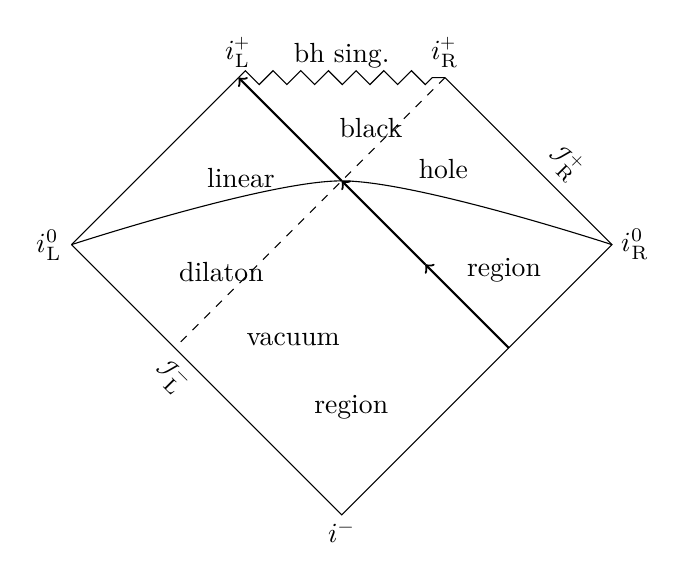
\begin{tikzpicture}%[scale=2]
\pgfmathsetmacro\myunit{3}
\pgfmathsetmacro\grs{0.6180339887498949}
\pgfmathsetmacro\grb{1.6180339887498949}
	\draw (0,0)
			node [left] {$i^0_\text{L}$}
		-- ++ (- 45: \grb * \myunit)
			node [pos = .50, below left, sloped] {$\mscrI^-_\text{L}$}
			node [pos = .10, right = .3*\myunit cm] {dilaton}
			node [pos = .35, right = .3*\myunit cm] {vacuum}
			node [pos = .60, right = .3*\myunit cm] {region}
			node [below] {$i^-$}
		-- ++ (+ 45: \myunit)
			%node [above = .25*\myunit cm] {region}
			coordinate (one)
		-- ++ (+ 45: \grs * \myunit)
			node [pos = .75, left = .15*\myunit cm] {region}
			node [right] {$i^0_\text{R}$}
			coordinate (r-inf)
		-- ++ (+135: \myunit)
			node [pos = .70, left = .35*\myunit cm] {black}
			node [pos = .45, left = .25*\myunit cm] {hole}
 			node [pos = .50, above right, sloped] {$\mscrI^+_\text{R}$}
			node [above] {$i^+_\text{R}$}
			coordinate (r-i+)
			;

	\draw (0,0)
		-- ++ (+ 45: \myunit)
			node [pos = .4, right = .25*\myunit cm] {linear}
			node [above] {$i^+_\text{L}$}
			coordinate (l-i+);
			%node [below = .55*\myunit cm] {linear}
			%node [below = .75*\myunit cm] {dilaton}
			%node [below = .95*\myunit cm] {vacuum};

	\draw [dashed] (r-i+)
		-- ++ (-135: \grb * \myunit)
			coordinate (mlambda);
		
	\draw [thick, ->] (one)
		-- ++ (+135: 0.5 * \myunit)
			coordinate (bb);
	\draw [thick, ->] (bb)
		-- ++ (+135: 0.5 * \myunit)
			coordinate (cross);
	\draw [thick, ->] (cross) -- (l-i+);

	\draw [decorate, decoration=zigzag] (l-i+)
		-- (r-i+)
		node [pos = .5, above] {bh sing.};

	\draw plot [smooth, dash dot] coordinates {(0,0) (cross) (r-inf)};
\end{tikzpicture}
\end{center}
\caption[Collapsing null matter in dilaton gravity]{The conformal 
diagram of collapsing null shell in $\rbr{1+1}$ dimensional dilaton gravity. 
The black-hole horizon is marked by the dashed line, whereas the ingoing null 
shell is expressed by the thick line with arrow. The \emph{linear dilaton 
vacuum region} and the \emph{black hole region} mark the space-time blocks 
before and after the ingoing shell, respectively. The quantum field, on the 
other hand, is solved on the hyper-surface connecting $i^0_\text{L/R}$ and the 
intersection of the null shell and the horizon.
\label{fig:dil-col-bod}}
\end{figure}

At the next-to-leading order in the semi-classical approximation scheme, the 
matter field can be separated from the gravity and the dilaton, and a quantum 
theory of fields in curved space-time can be \emph{derived} in terms of a 
functional Schrödinger equation
\begin{equation}
	\ii \frpa{\sfun{\chi}{f}}{t} = \int \dd x\,\frac{1}{2}
	\cbr{-\frdva{^2}{f^2} + \rbr{\frpa{f}{x}}^2} \sfun{\chi}{f},
\label{eq:functional-Sch-chi}
\end{equation}
where $\rfun{f}{x}$ is the classical matter field promoted to an operator, and 
$\sfun{\chi}{f}$ the corresponding matter wave-functional. Before the collapse 
of the ingoing null-matter-shell where the region is called \emph{linear dilaton 
vacuum}, a `vacuum' state can be found, whose wave functional reads
\begin{equation}
	\sfun{\chi_0}{f} \propto
	\cfun{\exp}{-\frac{1}{2}\int_{0}^{+\infty}\dd k\, k \, \rfun{f}{k}^2},
\label{eq:vacuum-wave-functional-f}
\end{equation}
where $\rfun{f}{k}$ is the Fourier sine transform of $\rfun{f}{x}$. 
\Cref{eq:vacuum-wave-functional-f} is nothing else but a generalisation of the 
ground-state wave function of a simple harmonic oscillator, see 
\cref{chap:harosc}.

After the collapse where the region is called \emph{black hole}, the spacial 
slice is shifted, and so are the Fourier modes of the matter field. It can be 
shown that
\begin{equation}
	\rfun{f}{k} = \int_{-\infty}^{+\infty} \dd l\,
	\rfun{\alpha}{k;l} \rfun{g}{l}\qquad k > 0,
\end{equation}
where $\rfun{g}{l}$ is the Fourier transform of matter field after the ingoing 
shock wave. The Bogolyubov-type coefficient $\rfun{\alpha}{k;l}$ has been 
computed, substituting which into \cref{eq:vacuum-wave-functional-f} yields
\begin{equation}
\sfun{\chi_b}{g} \propto 
\cfun{\exp}{-\int_{-\infty}^{+\infty}\dd p\, p \,\rfun{\coth}{\frac{\pp 
p}{2\lambda}} \vbr{\rfun{g}{p}}^2}
\label{eq:squeezed-wave-functional}
\end{equation}
in the black hole region, which is a squeezed-state wave functional 
\cite{Kiefer2001} and obviously different from a ground-state wave 
functional. The particle-number expectation of 
\cref{eq:squeezed-wave-functional} reads
\begin{equation}
	\abr{\rfun{n}{k}}_{\chi_b} = \rbr{\ee^{2\pp\vbr{k}/\lambda} - 1}^{-1},
	\label{eq:particle-num-exp-dilaton}
\end{equation}
%\begin{equation}
%\rfun{g}{k} = \int_{-\infty}^{+\infty}\dd v\,
%\frac{\ee^{-\ii k v}}{\sqrt{2\pp}} \rfun{f}{v},
%\end{equation}
leading to a Hawking-like \emph{black-body} temperature
\begin{equation}
T_\text{HD} \coloneqq \lambda/2\pp.
\label{eq:hawking-dilaton-temperature}
\end{equation}
Here it is the cosmological constant $\lambda$ which takes the place of surface 
gravity $\kappa$ in \cref{eq:hawking-temperature}.

%------------------------------------------------------------------------------
\section{Discussion}
\label{sec:hawrad-discussion}
%------------------------------------------------------------------------------

Though used throughout this work, the density operators can be mathematically 
defined only when they are \emph{trace-class} for which a trace may be defined, 
and this is not proved for any of the cases concerned. Unfortunately, the 
density operators are often not trace-class, especially in quantum field 
theory. A rigorous approach to deal with such thermal states can be the 
Kubo--Martin--Schwinger state \cite{Kubo1957,Martin1959,Haag1967} defined in 
algebraic quantum theory, which is concisely introduced in 
\cite[ch.~3]{David2015}.

Alert readers may be concerned about the result 
\cref{eq:squeezed-wave-functional}, which is derived in dilaton gravity model, 
not from Einstein gravitation. The solution is believed to be physically 
relevant, not only because it gives a same Hawking-like temperature for the CGHS 
black hole. It has also been shown that the wave functional of a massless, 
neutral scalar field in the Unruh effect yields exactly the same particle-number 
fluctuation and Hawking temperature \cite{Freese1985,Kiefer2001}. People have 
argued and widely believed that the Unruh effect is closely connected to 
Hawking radiation in Einstein gravity, especially in the space-time region near 
the horizon (e.g.\ \cite{Susskind2004}). It is therefore reasonable to believe 
that the aforementioned results from the CGHS model give hints about reality.

%%% Local Variables: 
%%% mode: latex
%%% TeX-master: "../mythesis"
%%% End: 

%==============================================================================
\chapter{Correlator of Field Strength}
\label{chap:corr_field}
%==============================================================================

Having revealed the discrepancy in the kinematic description of Hawking 
radiation, namely as either a pure or a thermal and mixed state, the author 
will show the difference in a physically relevant form. Recall that the 
particle-number expectations of the pure and mixed states are the same, 
i.e.\ the diagonal elements of the density operators in the particle-number 
basis are the same. Hence one seeks operators revealing the off-diagonal 
elements of the density operator.

%------------------------------------------------------------------------------
\section{Correlator and Fluctuation of Fourier Modes}
\label{sec:corr_Fourier}
%------------------------------------------------------------------------------

A natural candidate to reveal the off-diagonal elements of the density 
operators is the correlator. Bearing in mind the correlator of generalised 
Gaussian wave functions (see \cref{eq:multi-har-cor}), the correlator of the 
wave functional \cref{eq:squeezed-wave-functional} can be read off as
\begin{align}
\abr{\rfun{g^\dagger}{p_1}\rfun{g}{p_2}}_{\chi_b} &=
\frac{1}{2}\rbr{\abr{\rfun{g_\Re}{p_1}\rfun{g_\Re}{p_2}}_{\chi_b}+\abr{
\rfun{g_\Im}{p_1}\rfun{g_\Im}{p_2}}_{\chi_b}}
= \frac{1}{2}\frac{\tanh\frac{\pp p_1}{2\lambda}}{p_1} \rfun{\delta}{p_1 - 
p_2} \nonumber \\
&\propto \frac{1}{8T_\text{HD}}\frac{\rfun{\tanh}{q/4}}{q/4} = 
\frac{1}{8T_\text{HD}}\rbr{1 + \rfun{\Omicron}{q}}
\label{eq:correlator-pure}
\end{align}
by substituting
\begin{equation}
\rfun{g}{p} = 2^{-1/2} \rbr{\rfun{g_\Re}{p} + \ii \rfun{g_\Im}{p}},
\end{equation}
where $2^{-1/2}\rfun{g_\Re}{p}$ and $2^{-1/2}\rfun{g_\Im}{p}$ are the 
real and imaginary part of $\rfun{g}{p}$, respectively. In the last line of 
\cref{eq:correlator-pure}, the delta function is ignored, and the dimensionless 
parameter
\begin{equation}
	q \coloneqq p_1/T_\text{HD} \equiv 2\pp p_1/\lambda
\end{equation}
has been used. By the same argument, one also solves the correlator
\begin{equation}
\abr{\rfun{g^\dagger}{p_1}\rfun{g}{p_2}}_\text{vac} =
\frac{1}{2\vbr{p_1}}\rfun{\delta}{p_1-p_2} \propto
\frac{1}{2 T_\text{HD}} q^{-1}
\label{eq:correlator-vacuum}
\end{equation}
for the vacuum wave functional $\cfun{\exp}{-\int_{-\infty}^{+\infty}\dd p \, 
\vbr{p}\vbr{\rfun{g}{p}}^2}$.
%\begin{equation}
%\label{eq:vacuum-wave-functional-g}
%\end{equation}
For the thermal state, on the other hand, the correlator follows from
\cref{eq:correlator-multiple-thermal}, so that
\begin{align}
\abr{\rfun{g^\dagger}{p_1}\rfun{g}{p_2}}_\text{th} &=
\frac{\coth\frac{\pp p_1}{\lambda}}{2 p_1} \rfun{\delta}{p_1-p_2}
\nonumber \\
&\propto \frac{1}{4T_\text{HD}} \frac{\rfun{\coth}{q/2}}{q/2}
= \frac{1}{4T_\text{HD}}\rbr{\rbr{\frac{q}{2}}^{-2} + \frac{1}{3} + 
\rfun{\Omicron}{q}}.
\label{eq:correlator-thermal}
\end{align}

One sees immediately that 
\cref{eq:correlator-pure,eq:correlator-vacuum,eq:correlator-thermal} vanish 
identically for $p_1 \neq p_2$, which is due to the absence of interaction in 
the scalar field. The remaining diagonal terms have the meaning of 
\emph{fluctuation} in field strength, because $\abr{g} \equiv 0$, so that
\begin{equation}
	\abr{\rbr{\Delta g}^2} = \abr{g^2} - \abr{g}^2 \equiv \abr{g^2}.
\end{equation}
Ignoring the $\rfun{\delta}{0}$ divergence, the fluctuations are plotted in
\cref{fig:fluc-Fourier}.

\begin{figure}
\begin{center}
\begin{tikzpicture}
\begin{loglogaxis}[
xlabel = {$p \cdot T_\text{HD}^{-1}$},
extra x ticks = {3e-2, 3e-1, 3e0},
xticklabel={
        \pgfkeys{/pgf/fpu=true}
        \pgfmathparse{exp(\tick)}%
        \pgfmathprintnumber[fixed relative, precision=3]{\pgfmathresult}
        \pgfkeys{/pgf/fpu=false}
      },
ylabel = {$\abr{\vbr{\rfun{g}{p}}^2}\cdot T_\text{HD}$},
legend entries={vacuum,pure,thermal}]
\addplot[smooth]
table[x index = 0, y index = 1] {./graphics/mesh_fluc_fourier.dat};
\addplot[smooth, dashed]
table[x index = 0, y index = 2] {./graphics/mesh_fluc_fourier.dat};
\addplot[smooth, dashdotted]
table[x index = 0, y index = 3] {./graphics/mesh_fluc_fourier.dat};
\end{loglogaxis}
\end{tikzpicture}
\end{center}
\caption[Fluctuations of the Fourier modes]{Fluctuations of the Fourier modes 
of the field, plotted in log--log scales. The critical energy scale is the
Hawking temperature, below which the various fluctuations depart. The 
discrepancy between the pure and thermal descriptions is most significant for 
low-energy modes, while for high energies the fluctuations of them and 
the vacuum state are practically the same. Moreover, compared with vacuum, the 
low-energy fluctuation of thermal case is enhanced, so it diverges faster than 
that of vacuum; for the pure description, however, the fluctuation is 
suppressed, such that it converges to a constant of order unity and does not 
diverge any more. \label{fig:fluc-Fourier}}
\end{figure}

%------------------------------------------------------------------------------
\section{Discussion}
\label{sec:corr-discussion}
%------------------------------------------------------------------------------

It has been noticed that the fluctuation discussed above has been extensively 
used in cosmology, see e.g.\ \cite{Glenz2009}. The fluctuation in the 
radiation field, however, looks different from that in cosmology and thus 
remains yet to be explained.

Moreover, the most natural candidate to reveal the off-diagonal elements is the 
correlator in \emph{real space}, which is just the Fourier transform of the 
correlator calculated above. Unfortunately, the transformation has yet to be 
made for the thermal state due to an infra-red divergence.

%%% Local Variables: 
%%% mode: latex
%%% TeX-master: "../mythesis"
%%% End: 


%==============================================================================
\chapter{Quantification of the Difference}
\label{chap:quantifing}
%==============================================================================

Having shown explicitly the discrepancy between the pure and the thermal 
descriptions as well as where it is most significant, the author will then
quantify the difference. Related definitions of distances in quantum 
mechanics are introduced in \cref{chap:distappd}.
%In this chapter, it will be explained why the difference between the two cases 
%is expected to be negatively correlated to the mass of the black hole, then 
%the difference will be evaluated. 

%------------------------------------------------------------------------------
\section{The Canonical State} %Popescu--Winter Theorem
\label{sec:arbitrary-canonical}
%------------------------------------------------------------------------------

It has been shown in \cite{Popescu2006} that a small subsystem in a large, 
isolated system which is subject to a \emph{constraint}, is expected to be very 
close to a \emph{canonical state} of it, which reduces to the usual 
thermodynamic \emph{canonical ensemble} when the total system is under an 
\emph{energy constraint}.

Denoted by $U$, the large system has all its possible pure states in Hilbert 
space $\mscrH_U$ which has a finite dimension $d_R = \dim \mscrH_U$. A global 
constraint $R$ is also imposed, which restricts the physical Hilbert space of 
$U$ to $\mscrH_R \subseteq \mscrH_U$. The \emph{equiprobable state} of $U$ is
\begin{equation}
\mscrE_R \coloneqq d_R^{-1} \Bbbone_R,
\end{equation}
where $\Bbbone_R$ is the identity operator on $\mscrH_R$. An energy constraint, 
for instance, reads
\begin{equation}
\abr{H_U} = E_R,
\label{eq:ene-constraint}
\end{equation}
so that a state $\Ket{\alpha}$ in $\mscrH_R^{\rbr{\text{E}}}$ satisfies
\begin{equation}
E_R = \Braket{\alpha | H_U | \alpha} = \sum_E \vbr{\Braket{E | \alpha}}^2 E,
\end{equation}
where $\Ket{E}$ is an energy eigenstate of $U$ with eigenvalue $E$.

The subsystem in concern is named $S$, with \emph{all possible} states in the
Hilbert space $\mscrH_S$; the rest of $U$ is called the \emph{environment} and 
denoted by $E$, the pure states of which lie in $\mscrH_E$. One has
\begin{equation}
\mscrH_S \otimes \mscrH_E = \mscrH_U \supseteq \mscrH_R,\qquad
H_U = H_S + H_E + H_\text{int},
\end{equation}
where $H_S$, $H_E$ and $H_\text{int}$ are the system, environment and 
interaction Hamiltonian, respectively. 

The \emph{canonical state} of $S$ is defined as
\begin{equation}
{\Omega}_S \coloneqq \tr_E {\mscrE}_R,
\end{equation}
where the trace is taken over all the degrees of freedom in the environment. 
When the energy constraint \cref{eq:ene-constraint} is used, it can be shown 
that $\Omega_S^{(E)}$ is a canonical ensemble\footnote{A derivation of 
\cref{eq:canonical-state-def} in classical statistical physics can be found in 
\cite[sec.~28]{Landau1980}.}
\begin{equation}
\Omega_S^{(E)} \propto \ee^{- H_S/T_\text{m}}
= \sum_{E_S} \ee^{-E_S/T_\text{m}} \Ket{E_S}\Bra{E_S},
\label{eq:canonical-state-def}
\end{equation}
where $T_\text{m}$ can be identified with a temperature, and $\Ket{E_S}$ is an
eigenstate of the system with eigenvalue $E$. In this case it reduces to 
the traditional thermodynamic statistical physics.

%To state the theorems, one additional definition is needed: 
The environment also has an \emph{effective} dimension
\begin{equation}
d_E^\text{eff} \coloneqq \rbr{\tr \Omega_E^2}^{-1} \geq d_R/d_S,
\label{eq:def-effective-dim}
\end{equation}
where ${\Omega}_E = \tr_S {\mscrE}_R$. When no constraint is enforced, so that
$\mscrH_S \otimes \mscrH_E \equiv \mscrH_U = \mscrH_R$, 
\cref{eq:def-effective-dim} reduces to
\begin{equation}
d_E^\text{eff} = d_R/d_S = d_E.
\end{equation}
Detailed discussions about $d_E^\text{eff}$ can be found in \cite{Popescu2006}.

Equipped with all the definitions above, one picks an arbitrary pure state 
$\Ket{\phi}\in\mscrH_R$ and denote the \emph{reduced state} of $S$ by
\begin{equation}
\rfun{\rho_S}{\phi} = \tr_E \Ket{\phi}\Bra{\phi}
\end{equation}
Then a lemma states that the average \emph{trace distance}\footnote{See 
\cref{sec:trace-dist}.} between $\rho_S$ and $\Omega_S$ is very small in terms 
of the ratio between $d_S$ and $d_S/d_E^\text{eff}$, i.e.\
\begin{equation}
\abr{\rfun{T}{\rfun{\rho_S}{\phi}, {\Omega}_S}} \le \frac{1}{2}
\sqrt{\frac{d_S}{d_E^\text{eff}}}.
\end{equation}
In a typical division where $d_S/d_E$ is small, this average distance will also 
be tiny.

More over, the main theorem asserts that those ${\rho}_S$'s which are close to 
${\Omega}_S$ dominate; the probability of a large deviation is exponentially 
small with respect to the deviation. For an arbitrary $\epsilon > 0$, the 
theorem states that
\begin{equation}
\frac{\sfun{V}{\cbr{\Ket{\phi} \in \mscrH_R |
\rfun{T}{\rfun{\rho_S}{\phi}, \Omega_S} \geq \eta}}}
{\sfun{V}{\cbr{\Ket{\phi} \in \mscrH_R}}} \leq \eta',
\label{eq:main-theorem-Popescu}
\end{equation}
where
\begin{equation}
\eta = \epsilon + \frac{1}{2}\sqrt{\frac{d_S}{d_E^\text{eff}}}; \qquad
\eta' = 4\rfun{\exp}{-C d_R \epsilon^2},\quad C = \frac{2}{9\pp^3}.
\label{eq:main-theorem-supp}
\end{equation}
To understand the theorem, first note that the left-hand side of 
\cref{eq:main-theorem-Popescu} is a probability measure. More over, one can 
choose $\epsilon = d_R^{-1/3}$ as well, so that
\begin{equation}
\eta = \epsilon + \frac{1}{2}\sqrt{\frac{d_S}{d_E^\text{eff}}} \gtrsim 
d_R^{-1/3};\qquad
\eta' = 4\rfun{\exp}{-C d_R \epsilon^2} = 4\rfun{\exp}{-C d_R^{+1/3}},
\end{equation}
where $d_E^\text{eff} \gg d_S$ is also assumed. In this case, the probability 
of the deviation greater than $d_R^{-1/3}$ is smaller than an 
\emph{exponential} of $d_R^{+1/3}$.

Further explanations and proofs of the lemma and the theorem can 
be found in \cite{Popescu2006,Popescu2007}.

%------------------------------------------------------------------------------
\section{Distance between the Pure and Mixed States}
\label{sec:dist-radiation}
%------------------------------------------------------------------------------

To apply the aforementioned formalism to the Hawking radiation, one recognises 
the universe in the CGHS model as the total isolated system $U$, whereas the 
gravitational degrees of freedom as $E$, and the system in concern $S$ is the 
radiation field. It has been shown in \cite{Demers1996,Kiefer2001} that the 
reduced state of the radiation field can indeed be \emph{thermal} in certain 
\emph{decoherence} schemes, while in the collapsing case discussed in 
\cref{sec:hawrad-1+1dila,sec:1+1ddlt}, the radiation field remains pure.

In this section, the trace distance between the pure and thermal descriptions 
will be evaluated. Due to technical difficulties, the distance has not been able 
to be derived exactly. Instead, a lower and an upper bound have been set to the 
distance by \emph{Fuchs-van de Graaf inequality} in \cref{eq:ineq-fvdg}, where 
only the calculable \emph{Fidelity} (see \cref{sec:fidelity}) is needed.

Note that the wave functional of the Hawking radiation field 
\cref{eq:squeezed-wave-functional} is, roughly speaking, the superposition of 
quantum-mechanical wave functions per Fourier mode,
\begin{equation}
\sfun{\chi_b}{g} \sim \sum_p \rfun{\chi_b^\rbr{p}}{g_p}
= \sum_p \Braket{g_p | \chi_b^\rbr{p}},
\label{eq:wave-function-decomposed}
\end{equation}
where $g_p \coloneqq \rfun{g}{p}$ is the Fourier transform of the field $g$ 
evaluated at $p$. On the other hand, the thermal state of the free field can 
also be sloppily written as the product of the quantum-mechanical density 
operators per mode,
\begin{equation}
{\rho}_\text{th} \sim \bigotimes_p {\rho}_\text{th}^\rbr{p}.
\end{equation}
By \cref{eq:fidelity-pure-mixed}, the fidelity of $\sfun{\chi_b}{g}$ and 
$\rho_\text{th}$ can be reduced to the product of the fidelity per mode, because
\begin{equation}
\Braket{\chi_b | {\rho}_\text{th} | \chi_b} \sim \prod_p 
\Braket{\chi_b^\rbr{p} | {\rho}_\text{th}^\rbr{p} | \chi_b^\rbr{p}}.
\label{eq:expectation-decomposed}
\end{equation}

Since $\Ket{\chi_b^\rbr{p}}$ is just a quantum-mechanical general Gaussian 
state (see \cref{sec:single-harosc}), the result in \cref{eq:fidelity-gg-th} 
can be adapted by substituting
\begin{equation}
\Omega = \vbr{p},\qquad \omega = p\,\coth\frac{\pp p}{2\lambda}\quad
\text{and}\quad T = T_\text{HD} \equiv \frac{\lambda}{2\pp},
\end{equation}
yielding the \emph{fidelity per mode}
\begin{equation}
F^\rbr{p} = \frac{\sqrt{u-1}}{\sqrt[4]{u^2+u+1}},\qquad
u \coloneqq \ee^q \equiv \ee^{\vbr{p}/T_\text{HD}},
\label{eq:fidelity-pt}
\end{equation}
so that the trace distance per Fourier mode can be evaluated, see 
\cref{fig:trace-dist-per-mode}.

\begin{figure}
\begin{center}
\begin{tikzpicture}
\begin{semilogyaxis}[
xlabel = {$p \cdot T_\text{HD}^{-1}$},
ylabel = {$\rfun{T}{\Ket{p}, \rfun{\rho_\text{th}^\rbr{p}}{T_\text{HD}}}$},
legend entries={\small lower bound, \small upper bound,
\small possible value},
legend pos = south west]
\addplot[name path = lower, smooth, dashed]
	table [x index = 0, y index = 1] 
		{./graphics/mesh_trace_dist_mode_bounds.dat};
\addplot[name path = upper, smooth, dotted]
	table [x index = 0, y index = 2] 
		{./graphics/mesh_trace_dist_mode_bounds.dat};
\addplot[gray!50]
	fill between [of = lower and upper];
\end{semilogyaxis}

\end{tikzpicture}
\end{center}
\caption[Possible value of the trace distance per Fourier mode]{Possible value 
of the trace distance between mode wave functions in 
\cref{eq:wave-function-decomposed} and the corresponding thermal density 
operators. One sees that the difference becomes exponentially small with respect 
to $p/T_\text{HD}$, which suggests it would be difficult to distinguish the pure 
and thermal descriptions by detecting the high-energy modes in the Hawking 
radiation, confirming the results in \cref{sec:corr_Fourier}.
\label{fig:trace-dist-per-mode}}
%, evaluated in terms of lower and upper bound by fidelity
\end{figure}

To approach the trace distance for the wave functional and the total thermal 
state, one needs to deal with the product with continuous index in 
\cref{eq:expectation-decomposed}. A popular way to go to the `continuous limit' 
in \emph{summation} is
\begin{equation}
\sum_p \rfun{g}{p} \to \frac{1}{2\pp\Lambda} \int \dd p\,\rfun{g}{p},
\end{equation}
where $\Lambda$ has the same dimension as $p$ in order to fix the dimension; in 
the box-normalisation scheme, for example, the corresponding $\Lambda$ would be 
proportional to the volume of the box $V$. A similar method may be used to 
normalise the product, namely
\begin{equation}
\prod_p \rfun{f}{p} = \cfun{\exp}{\sum_p \ln\rfun{f}{p}} \to 
\cfun{\exp}{\frac{1}{2\pp\Lambda}\int \dd p\,\ln\rfun{f}{p}}.
\end{equation}
Note that the wave functional \cref{eq:squeezed-wave-functional}, which has 
always been dealt with, can also be seen as being normalised by the method.
One thus derives
\begin{equation}
F = \cfun{\exp}{\frac{2}{2\pp\Lambda}\int_0^{+\infty}\dd p\,\ln F^\rbr{p}}
= \rfun{\exp}{-\frac{\pp}{9} \frac{T_\text{HD}}{\Lambda}},
\end{equation}
which is shown in \cref{fig:trace-dist-total}.

\begin{figure}
\begin{center}
\begin{tikzpicture}
\begin{loglogaxis}[
xlabel = {$T_\text{HD} \cdot \Lambda^{-1}$},
extra x ticks = {3e-2, 3e-1, 3e0},
xticklabel={
        \pgfkeys{/pgf/fpu=true}
        \pgfmathparse{exp(\tick)}%
        \pgfmathprintnumber[fixed relative, precision=3]{\pgfmathresult}
        \pgfkeys{/pgf/fpu=false}
      },
ylabel = {$\rfun{T}{\chi_b, \rfun{\rho_\text{th}}{T_\text{HD}}}$},
extra y ticks = {3e-1, 3e-2},
yticklabel={
        \pgfkeys{/pgf/fpu=true}
        \pgfmathparse{exp(\tick)}%
        \pgfmathprintnumber[fixed relative, precision=3]{\pgfmathresult}
        \pgfkeys{/pgf/fpu=false}
      },
legend entries={
\small lower bound,
\small upper bound,
\small possible value},
legend pos = south east]
\addplot[name path = lower, smooth, dashed]
	table [x index = 0, y index = 1] 
		{./graphics/mesh_trace_dist_total_bounds.dat};
\addplot[name path = upper, smooth, dotted]
	table [x index = 0, y index = 2] 
		{./graphics/mesh_trace_dist_total_bounds.dat};
\addplot[gray!50]
	fill between [of = lower and upper];
\end{loglogaxis}

\end{tikzpicture}
\end{center}
\caption[Possible value of the trace distance between pure and thermal 
descriptions]{Possible value of the trace distance between the pure and thermal 
descriptions of the Hawking radiation field. One sees that the difference 
between the two cases is positively (negatively) correlated with the Hawking 
temperature temperature (mass of black hole). 
\label{fig:trace-dist-total}}
\end{figure}

%------------------------------------------------------------------------------
\section{Discussion}
\label{sec:dist-discussion}
%------------------------------------------------------------------------------
Strictly speaking, the formalism in \cref{sec:arbitrary-canonical} is \emph{not}
applicable to the radiation field considered here, because they were proved for 
\emph{finite dimensional systems}, while the cases in this work are all 
\emph{infinite-dimensional}. However, since a regularised result can be 
obtained, it is believable that a mathematically rigorous approach exists, which 
will justify the result, similar to the renormalisation procedure in quantum 
field theory.

Though the asymptotic behaviour of the trace distance with respect to Hawking 
temperature has clearly been revealed by setting bounds to it, it is still 
appealing to calculate its \emph{exact value}. One possible approach is by 
using the results in \cite{Joos1985}, where the eigenfunctions and eigenvalues 
of a general Gaussian density operator have been explicitly solved.

The evaluation of the trace distance was motivated by \citeauthor{Hsu2009} in 
\cite{Hsu2009}, where operational meaning of the distance was also discussed in 
terms of toy models, which is unfortunately not applicable to the field system. 
In future works, it is expected that the distance between the pure and thermal 
states will be understood in terms of \emph{experiments} or \emph{observations}, 
where the essence of physical science lies.


%%% Local Variables: 
%%% mode: latex
%%% TeX-master: "../mythesis"
%%% End: 


%==============================================================================
\chapter{Summary and Outlook}
\label{chap:summary}
%==============================================================================

In this work, the discrepancy of the pure-state and thermal descriptions of 
Hawking radiation field has been revealed, based on the CGHS gravity model. It 
has been shown that in fluctuations of Fourier modes, the difference is 
significant for low-energy excitations while vanishing for high-energy ones, 
which fits the result that the Hawking-radiation particles are mostly 
low-energetic, compared with the Hawking temperature. Moreover, motivated by the 
new foundation of statistical physics, the discrepancy between the two 
descriptions has been quantified and proved to be large for a low-mass 
black hole, which is expected to show more traces of quantum gravity.

The CGHS model used throughout is only one of the solvable alternative gravity 
models. One may further attempt other popular choices, for example, the 
\emph{Bañados--Teitelboim--Zanelli model} \cite{Banados1992} in $\rbr{2+1}$ 
dimensions, and compare the relevant results.

Equipped with the results in the thesis, one expects deeper understandings 
about the nature of the black-hole entropy and the final fate of the black-hole 
evaporation, which have been in the spotlight since the advent of Hawking 
radiation.

In future works, the decoherence formalism will also be taken into account, in 
which a thermalised reduced state of the radiation field can be obtained 
explicitly.
% Uncomment the following command to get references per chapter.
% Put it inside the file or change \include to \input if you do not want the references
% on a separate page
% \printbibliography[heading=subbibliography]

%------------------------------------------------------------------------------
% Use biblatex for the bibliography
% Add bibliography to Table of Contents
% Comment out this command if your references are printed for each chapter.
\printbibliography[heading=bibintoc]

%------------------------------------------------------------------------------
% Include the following lines and comment out \printbibliography if
% you use BiBTeX for the bibliography.
% If you use biblatex package the files should be specified in the preamble.
% \KOMAoptions{toc=bibliography}
% {\raggedright
%   \bibliographystyle{../refs/atlasBibStyleWithTitle.bst}
%   % \bibliographystyle{unsrt}
%   \bibliography{./thesis_refs,../refs/standard_refs-bibtex}
% }

%------------------------------------------------------------------------------
\appendix
% \part*{Appendix}
% Add your appendices here - don't forget to also add them to \includeonly above
%%------------------------------------------------------------------------------
%\chapter{Useful information}
%\label{sec:app}
%------------------------------------------------------------------------------

In the appendix you usually include extra information that should be
documented in your thesis, but not interrupt the flow.

%\chapter{Classical gravitations}

\section{Einstein gravitation}

\section{Dilaton gravitation}

%\chapter{Quantum aspects of gravitation}

\section{Quantum fields with Einsteinian background}

\section{Quantized dilaton gravitation}

%%% Local Variables: 
%%% mode: latex
%%% TeX-master: "../mythesis"
%%% End: 

%==============================================================================
\chapter{$\rbr{1+1}$-dimensional Dilaton Gravity}
\label{sec:1+1ddlt}
%==============================================================================

Since quantum field theories in $\rbr{3+1}$-dimensional Einstein gravitation 
are difficult to solve, one may turn to alternative solvable gravity models to 
get some hints for the physics in reality. The $\rbr{1+1}$-dimensional dilaton 
gravity, or the Callan--Giddings--Harvey--Strominger (CGHS) model, is such a 
candidate, which is used in the thesis and has been extensively studied in the 
literature, see for instance \cite{Callan1992,Demers1996,Ashtekar2011}. In this 
chapter a very brief review of the model is provided, mainly based on 
\cite{Demers1996}.

The action for the model, with $N$ massless scalar fields minimally coupled, 
reads
\begin{equation}
S \coloneqq \int \dd^2 x \sqrt{-\ol{g}}\cbr{\frac{\ee^{-2\ol{\phi}}}{\nG}
\sbr{\ol{R}+4\rbr{\nabla \ol{\phi}}^2 + 4\lambda^2}
-\frac{1}{2}\sum_{i=1}^N\rbr{\nabla f_i}^2},
\label{eq:action-CGHS-dilaton}
\end{equation}
where $f_i$'s are the neutral scalar matter fields, $\ol{\phi}$ is the dilaton 
field, $\nG$ the dimensionless Newton constant, and $\lambda > 0$ the 
cosmological constant. The dilaton field is essential in two dimensions, because 
there is only one independent component in the Riemann curvature tensor, hence a 
pure $\rbr{1+1}$-dimensional Einstein theory shall be trivial. Transforming 
with $\phi = \ee^{-2\ol{\phi}}$ and $g_{\alpha\beta} = \ee^{-2\ol{\phi}} 
\ol{g}_{\alpha\beta}$ eliminates the kinetic term for the dilaton, yielding
\begin{equation}
S = \int \dd x\,\dd t\sqrt{-g}\cbr{\frac{1}{\nG}\sbr{R\phi + 4\lambda^2}
-\frac{1}{2}\rbr{\nabla f}^2},
\label{eq:action-CGHS-dilaton-eli}
\end{equation}
where only one matter field is considered for simplicity, and an 
ADM-like\footnote{Arnowitt--Deser--Misner, see \cite{Arnowitt2008}.}
parametrisation of the metric
\begin{equation}
\dd s^2 = \ee^{2\rho}\sbr{-\sigma^2\,\dd t^2 + \rbr{\dd x + \xi\,\dd t}^2}
\label{eq:ADM-para}
\end{equation}
is assumed, in which $\rbr{\sigma, \xi}$ are the lapse and shift functions.
The action in \cref{eq:action-CGHS-dilaton-eli} has a classical solution 
describing a collapsing null-matter shell, which resembles the solution of 
a spherically collapsing body in the $\rbr{3+1}$-dimensional Einstein case. 
The corresponding conformal diagram is plotted in \cref{fig:dil-col-bod}.

To apply the canonical quantisation scheme, the action in
\cref{eq:action-CGHS-dilaton-eli} is to be recast in the Hamiltonian formalism.
However, the Legendre transformation of the field momenta proves to be 
singular. This means that the momenta, as functions of the positions and 
velocities, cannot be inverted to express the corresponding velocities as 
functions of momenta and positions, so that the standard algorithm to obtain 
the Hamiltonian
\begin{equation}
H \coloneqq \sbr{\frpa{L}{\dot{X}_i}\dot{X}_i - L}_{\dot{X}
= \rfun{\dot{X}}{P,X}}
\end{equation}
does not apply, where $\rbr{X, \dot{X}, P}$ are the positions, velocities and 
momenta, respectively.

The systems, of which the Legendre transformation is singular, are called 
\emph{constrained systems}. Other examples include a relativistic point 
particle in the covariant form, Yang--Mills theories and string theories. For 
such systems, the usual quantisation scheme and the Schrödinger equation do 
not apply directly. Instead, one has to identify the constraints in the system 
and apply Dirac's quantisation rules \cite{dirac1964lectures,Gitman1990}. The 
result is that the quantum wave functional describing the CGHS model is 
\emph{constrained} by
\begin{align}
0 = \mscrH_\parallel\sfun{\Psi}{\rho,\phi,f} &\coloneqq
\rbr{\frde{\rho}{x}\frdva{}{\rho} - \frde{}{x}\frdva{}{\rho} 
+\frde{\phi}{x}\frdva{}{\phi} + \frde{f}{x}\frdva{}{f}}\sfun{\Psi}{\rho,\phi,f},
\label{eq:hpara}\\
0 = \mscrH_\perp\sfun{\Psi}{\rho,\phi,f} &\coloneqq
\rbr{\frac{\nG}{2}\frdva{^2}{\rho\,\dva\phi} - \frac{1}{2}\frdva{^2}{f^2} 
+\frac{1}{2\nG}V_G + V_M}\sfun{\Psi}{\rho,\phi,f},
\label{eq:hperp}
\end{align}
where
\begin{equation}
V_G \coloneqq 4\rbr{\frde{^2\phi}{x^2} - \frde{\phi}{x}\frde{\rho}{x} - 
2\lambda^2 \ee^{2\rho}},\qquad
V_M \coloneqq\frac{1}{2}\rbr{\frde{f}{x}}^2.
\end{equation}
\Cref{eq:hpara,eq:hperp} are the \emph{Wheeler--DeWitt equations} for the CGHS 
model, which play the role of the usual Schrödinger equation for the whole 
system.

In the next step, a semi-classical approximation (see also \cite[sec.\ 
5.4]{Kiefer2012}) of the Born--Oppenheimer type is applied to $\Psi$ by 
expanding the exponent as
\begin{equation}
\sfun{\Psi}{\rho,\phi,f} = \ee^{\ii\rbr{\nG^{-1}S_0 + S_1 + \nG S_2 + \ldots}}.
\end{equation}
Inserting this expression into \cref{eq:hpara,eq:hperp}, one finds that at 
order $\nG^{0}$, variables can be separated by setting
\begin{equation}
\ee^{\ii S_1} \coloneqq \sfun{D^{-1}}{\rho,\phi}\sfun{\chi}{\rho,\phi,f}.
\end{equation}
Inserting the leading and next-to-leading order terms into 
\cref{eq:hpara,eq:hperp} yields
\begin{equation}
\ii \rbr{\frpa{\rho}{t}\frdva{\chi}{\rho} + \frpa{\phi}{t}\frdva{\chi}{\phi}} = 
\frac{1}{2}\cbr{-\frdva{^2}{f^2}+\rbr{\frpa{f}{x}}^2} \chi,
\end{equation}
integrating of which gives the functional Schrödinger equation for the matter 
field \eqref{eq:functional-Sch-chi}.


% Order $\nG^{-1}$: Hamilton--Jacobi for pure gravity


%%% Local Variables: 
%%% mode: latex
%%% TeX-master: "../mythesis"
%%% End: 

%==============================================================================
\chapter{Harmonic Oscillators}
\label{chap:harosc}
%==============================================================================

%------------------------------------------------------------------------------
\section{Single Harmonic Oscillator}
\label{sec:single-harosc}
%------------------------------------------------------------------------------

A single harmonic oscillator is described by the Hamiltonian
\begin{equation}
H = \frac{1}{2}\rbr{\pi^2 + \Omega^2f^2},
\label{eq:hamiltonian-simple-harosc}
\end{equation}
where $\rbr{\pi, f}$ are conjugate momentum and position, respectively. Here
a unit system similar to the case in field theory is adapted. Canonical
quantisation uses the annihilation and creation operators
\begin{equation}
a^- \coloneqq \frac{1}{\sqrt{2}}\rbr{\sqrt{\Omega}f + 
\frac{\ii}{\sqrt{\Omega}}\pi}, \qquad
a^+ \coloneqq \frac{1}{\sqrt{2}}\rbr{\sqrt{\Omega}f
-\frac{\ii}{\sqrt{\Omega}}\pi} \equiv \rbr{a^-}^\dagger;
\end{equation}
inverse expressions read
\begin{equation}
f = \frac{a^++a^-}{\sqrt{2\Omega}},\qquad
\pi = \ii\sqrt{\frac{\Omega}{2}}\rbr{a^+-a^-}.
\end{equation}
The ground state and the normalised $n$th excitation are defined by
\begin{equation}
a^-\Ket{0} \coloneqq 0,\qquad
\Ket{n} \coloneqq \frac{1}{\sqrt{n!}}\rbr{a^+}^n\Ket{0},\qquad
n \in \BbbZ_+,
\end{equation}
the wave functions of which are
\begin{equation}
\Braket{f | n} = \frac{1}{\sqrt{2^n n!}} 
\ee^{-\Omega f^2/2} \rfun{H_n}{\sqrt{\Omega}f}, \qquad
n \in \BbbZ,
\end{equation}
where $\rfun{H_n}{x}$ is the $n$th Hermite polynomial. The normalising measure
\begin{equation}
\rfun{\dd \mu}{f} \coloneqq \sqrt{\frac{\Omega}{\pp}}\,\dd f
\end{equation}
is used throughout, so that the completeness relation holds,
\begin{align}
\int \rfun{\dd \mu}{f}\,\Braket{\alpha | f}\Braket{f | \beta} \equiv
\Braket{\alpha | \beta}.
\end{align}

In the present work, a general Gaussian state $\Ket{\omega}$ has also been 
considered, the wave function of which reads
\begin{equation}
\Braket{f | \omega} = \rbr{\frac{\Re\omega}{\Omega}}^{1/4}
\rfun{\exp}{-\frac{\omega}{2}f^2},\qquad \Re \omega > 0
\label{eq:general-single-omega}
\end{equation}
Evaluating the expectation of $f^2$ yields
\begin{equation}
\abr{f^2}_\omega \coloneqq \Braket{\omega | f^2 | \omega}
= \rbr{2\Re \omega}^{-1}.
\label{eq:correlator-1}
\end{equation}
$\Ket{\omega}$ can also be expressed in terms of energy eigenstates,
\begin{align}
\Braket{n | \omega} &= \int \rfun{\dd \mu}{f}\, \Braket{n | f} 
\Braket{f | \omega} \nonumber \\
&= \rbr{\frac{\Omega \Re\omega}{\pp^2}}^{1/4} \frac{1}{\sqrt{2^n n!}}
\int_{-\infty}^{+\infty} \dd f\,
\cfun{\exp}{-\frac{1}{2}\rbr{\Omega+\omega}f^2}\rfun{H_n}{\sqrt{\Omega}f}
\nonumber \\
&= \begin{cases} \rbr{\Omega  \Re(\omega )}^{\frac{1}{4}}
\dfrac{2^{\frac{1}{2}-m} \sqrt{(2 m)!} }{m!}
\dfrac{(\Omega -\omega )^m}{(\omega +\Omega )^{m+\frac{1}{2}}}
& n = 2m, \\
0 & n = 2m+1,
\end{cases}
\label{eq:n|omega}
\end{align}
thanks to \cite{Babusci2012}.

A thermal state of the oscillator at temperature $T$ can be described by the
density operator
\begin{equation}
\rho \coloneqq \frac{1}{Z} \cfun{\exp}{-\frac{H}{T}} = \frac{1}{Z} 
\sum_{n=0}^{+\infty} \cfun{\exp}{-\frac{\Omega}{T}\rbr{n+\frac{1}{2}}} 
\Ket{n}\Bra{n},
% \nonumber \\
%&= Z^{-1} \sum_{n=0}^{+\infty} 
%\frac{\ee^{-\frac{\Omega}{T}\rbr{n+\frac{1}{2}}}}{n!}
%\rbr{a^+}^n\Ket{0}\Bra{0}\rbr{a^-}^n,
\label{eq:single-thermal-density-mat}
\end{equation}
where the partition function is
\begin{equation}
Z \coloneqq \tr{\ee^{-H/T}} = \frac{1}{2} \csch\frac{\Omega}{2 T}.
\end{equation}
One also obtains
\begin{align}
\abr{f^2}_\rho &= \frac{1}{2\Omega}\frac{1}{Z}\sum_{n=0}^{+\infty}
\cfun{\exp}{-\frac{\Omega}{T}\rbr{n+\frac{1}{2}}}
\Braket{n | \rbr{a^++a^-}^2 | n} \nonumber \\
%&= \frac{1}{2\Omega}\frac{1}{Z}\sum_{n=0}^{+\infty}
%\ee^{-\frac{\Omega}{T}\rbr{n+\frac{1}{2}}}
%\Braket{n | \rbr{\rbr{a^+}^2+a^+a^-+a^-a^++\rbr{a^-}^2} | n} \nonumber \\
&= \frac{1}{2\Omega}\frac{1}{Z}\sum_{n=0}^{+\infty}
\cfun{\exp}{-\frac{\Omega}{T}\rbr{n+\frac{1}{2}}}
\Braket{n | \rbr{2a^+a^-+1} | n} %\nonumber \\
%&= \frac{\coth\frac{\Omega}{2 T}}{2\Omega}
= \frac{1}{4T} \frac{\coth\frac{\Omega}{2 T}}{\frac{\Omega}{2 T}}.
\label{eq:sho-th-cor-1}
\end{align}
%\Cref{eq:single-thermal-density-mat} expressed in terms of position basis can
%also be calculated
%\begin{align}
%\rho &= \frac{1}{Z}
%\sum_{n=0}^{+\infty} \ee^{-\frac{\Omega}{T}\rbr{n+\frac{1}{2}}}
%\int\rfun{\dd\mu}{f_1}\,\rfun{\dd\mu}{f_2}\,
%\Ket{f_1}\Braket{f_1 | n}\Braket{n | f_2}\Bra{f_2}
%\nonumber \\
%&= \frac{1}{Z} \int\rfun{\dd\mu}{f_1}\,\rfun{\dd\mu}{f_2}\,\Ket{f_1}
%\rbr{\sum_{n=0}^{+\infty}\ee^{-\frac{\Omega}{T}\rbr{n+\frac{1}{2}}}
%\Braket{f_1 | n}\Braket{n | f_2}}
%\Bra{f_2};
%\label{eq:thermal-position-basis-1}
%\end{align}
%The summation in \cref{eq:thermal-position-basis-1} can be closed
%\begin{equation}
%\rfun{\dd\mu}{f_1}\,\rfun{\dd\mu}{f_2}\,
%\sum_{n=0}^{+\infty}\Braket{f_1 | n}\Braket{n | f_2}
%= \dd f_1\,\dd f_2 \rfun{\delta}{f_1 - f_2},
%\end{equation}
%due to orthonormality and completeness of the bases.

%------------------------------------------------------------------------------
\section{Multiple Harmonic Oscillators}
%------------------------------------------------------------------------------

Multiple harmonic oscillators are described by the Hamiltonian
\begin{equation}
H = \sum_i H_i,\qquad H_i = \frac{1}{2}\rbr{\pi_i^2 + \Omega^2f_i^2},
\end{equation}
where $\rbr{\pi_i, f_i}$ are conjugate momentum and position of the $i$th
oscillator.

When the general Gaussian state
\begin{equation}
\Braket{\cbr{f} | \sbr{\omega}} = \rbr{\det\frac{\omega}{\Omega}}^{1/4} 
\rfun{\exp}{-\frac{1}{2}f_i \omega_{ij} f_j}
\label{eq:general-ij-omega}
\end{equation}
is considered, where $\omega_{ij}$ is a real symmetric positive-definite
matrix, the two-point correlator becomes
\begin{equation}
\Braket{\sbr{\omega} | f_i f_j | \sbr{\omega}} = \sbr{\rbr{2\omega}^{-1}}_{ij},
\label{eq:multi-har-cor}
\end{equation}
which is a generalisation of \cref{eq:correlator-1}.

A thermal state at temperature $T$ can be described by the density operator
\begin{equation}
\rho = \bigotimes_i \rho_i,\qquad \rho_i =
\frac{1}{Z} \rfun{\exp}{-\frac{H_i}{T}}.
\label{eq:multi-thermal-density-mat}
\end{equation}
Computing the two-point correlator of the state, one finds
\begin{equation}
\abr{f_if_j}_\rho = \frac{\coth\frac{\Omega_i}{2T}}{2\Omega_i}
\delta_{ij}
= \frac{1}{4T} \frac{\coth\frac{\Omega_i}{2T}}{\frac{\Omega_i}{2T}} 
\delta_{ij}
\label{eq:correlator-multiple-thermal}
\end{equation}
from \cref{eq:sho-th-cor-1}.

%%% Local Variables: 
%%% mode: latex
%%% TeX-master: "../mythesis"
%%% End: 

%==============================================================================
\chapter{Distances in Quantum Theory}
\label{chap:distappd}
%==============================================================================

This chapter follows mostly \cite{Wilde2009}. Some conventions follow those in 
\cite{Petz2008}.

%------------------------------------------------------------------------------
\section{Trace Distance}
\label{sec:trace-dist}
%------------------------------------------------------------------------------

To begin with, define the \emph{trace norm} or \emph{$l_1$-norm} of an 
Hermitian operator $M$ as
\begin{equation}
	\dvbr{M}_1 \coloneqq \tr\sqrt{M^\dagger M}.
\end{equation}
When the spectral decomposition $M = \sum_i \mu_i \Ket{i}\Bra{i}$ exists, the 
trace norm reads
\begin{equation}
	\dvbr{M}_1 \equiv \sum_i\vbr{\mu_i},
\end{equation}
so the name $l_1$-norm comes. It is positive definite and homogeneous; the 
triangle inequality also holds. Thus it can be used to define the \emph{trace 
distance} between Hermitian operators ${M}$ and ${N}$ as
\begin{equation}
\rfun{T}{{M}, {N}} \coloneqq \frac{1}{2} \dvbr{M-N}_1 \equiv
\frac{1}{2} \tr \sqrt{\rbr{{M}-{N}}^\dagger\rbr{{M}-{N}}}.
\label{eq:def-trace-dist}
\end{equation}
Now consider density operators $\rho$ and $\sigma$ only. Since $\dvbr{\rho}_1 
\equiv 1$, one sees
\begin{equation}
0 \le \rfun{T}{{\rho}, {\sigma}} \le 1,
\label{eq:def-trace-prop}
\end{equation}
followed from positive definiteness and triangle inequality.

The following lemma helps constructing a physical interpretation of the 
distance. Let the Hermitian operator $\Lambda$ be such that all its eigenvalues 
lies within $\sbr{0,1}$, then
\begin{equation}
\rfun{T}{{\rho}, {\sigma}} = \max_{0 \le {\Lambda} \le \Bbbone}
\cfun{\tr}{{\Lambda}\rbr{{\rho}-{\sigma}}}.
\end{equation}
To understand this, take $\Lambda \equiv \Ket{\alpha}\Bra{\alpha}$,
where $\Ket{\alpha}$ is the eigenket of some observable $\Alpha$, with 
eigenvalue $\alpha$. Then $\tr\cbr{\Lambda \rho}$ tells the probability of 
measuring $\Alpha$ which gives the result $\alpha$. Therefore $\tr\cbr{\Lambda 
\rbr{\rho-\sigma}}$ gives the difference of the probability above for $\rho$ and 
$\sigma$, and $\rfun{T}{{\rho}, {\sigma}}$ is the maximal value of the 
difference above.

Though the trace distance is used in formulating \cref{chap:quantifing}, it is 
rather formidable to compute due to the operatorial square root in 
\cref{eq:def-trace-dist}. Therefore the author seeks other ways to evaluate the 
quantity.

%------------------------------------------------------------------------------
\section{Fidelity}
\label{sec:fidelity}
%------------------------------------------------------------------------------

Fidelity is another means to compare two quantum states. The simplest case 
of fidelity is that of two pure states,
\begin{equation}
\rfun{F}{\Ket{\alpha},\Ket{\beta}} \coloneqq \vbr{\Braket{\alpha | \beta }}.
\end{equation}
One sees that it is just the modulus of the transition amplitude, a measure of 
\emph{faithfulness}. For more general cases, fidelity is defined as
\begin{align}
\rfun{F}{\Ket{\alpha},{\sigma}} &\coloneqq \sqrt{\Braket{\alpha | {\sigma} | 
\alpha}}, \\
\label{eq:fidelity-pure-mixed}
\rfun{F}{{\rho},{\sigma}} &\coloneqq \tr\sqrt{{\rho}^\frac{1}{2} 
{\sigma} {\rho}^\frac{1}{2}}.
\end{align}
In applications in this work, fidelity is solvable because only
\cref{eq:fidelity-pure-mixed} is needed.

An important property of fidelity is that it follows the \emph{Fuchs--van de 
Graaf inequality} \cite{Fuchs1999})
\begin{equation}
1 - \rfun{F}{{\rho},{\sigma}} \le \rfun{T}{{\rho},{\sigma}}
\le \sqrt{1 - \rfun{F^2}{{\rho},{\sigma}}}.
\label{eq:ineq-fvdg}
\end{equation}
In this work, the trace distances are evaluated by computing the fidelities 
exactly and inserting them to \cref{eq:ineq-fvdg}.

Consider a single harmonic oscillator with intrinsic frequency $\Omega$, a 
thermalised state of it at temperature $T$ described by a density operator 
$\rfun{\rho}{T}$, as well as a generalised Gaussian state $\Ket{\omega}$ (see 
\cref{sec:single-harosc}). In the following the fidelity of them will be 
calculated.

Since $\rfun{\rho}{T}$ is diagonal in the energy-eigenstate basis $\Ket{n}$, one 
has
\begin{equation}
\Braket{\omega | \rfun{\rho}{T} | \omega} = \sum_{n=0}^{+\infty}
\Braket{\omega | n} \Braket{n | \rfun{\rho}{T} | n} \Braket{n | \omega},
\label{eq:fidelity-1}
\end{equation}
in which
\begin{align}
\Braket{n | \omega} &= 
\begin{cases} \rbr{\Omega  \Re\omega }^{\frac{1}{4}}
\dfrac{2^{\frac{1}{2}-m} \sqrt{(2 m)!} }{m!}
\dfrac{(\Omega -\omega )^m}{(\omega +\Omega )^{m+\frac{1}{2}}}
& n = 2m, \\
0 & n = 2m+1,
\end{cases}
\tag{\ref{eq:n|omega} revisited} \\
\Braket{n | \rho | n} &=
\frac{1}{Z}\cfun{\exp}{-\rbr{n+\frac{1}{2}}\frac{\Omega}{T}}
\equiv 
\rbr{\ee^{\Omega/T}-1} \cfun{\exp}{-\rbr{n+1}\frac{\Omega}{T}}.
\label{eq:n|rho|n}
\end{align}
Inserting \cref{eq:n|omega,eq:n|rho|n} into \cref{eq:fidelity-1}, one finds 
that each term in the summation is of the form $b\cdot\binom{2m}{m}a^{2m}$ 
where $a$ and $b$ are expressions of $\Omega$, $\omega$ and $T$, which can be 
computed by using
\begin{equation}
\arcsin z = \sum_{n=0}^{+\infty} \binom{2n}{n}\frac{z^{2n+1}}{4^n\rbr{2n+1}}
\end{equation}
and taking derivative with respect to $z$ on both sides. Therefore the fidelity 
of $\rho(T)$ and $\Ket{\omega}$ is computed to be
\begin{equation}
\rfun{F}{\Ket{\omega}, \rho(T)} = \sqrt{2} \sqrt[4]{\frac{\Omega  \Re{\omega} 
\left(\ee^{\Omega /T}-1\right)^2}{(\Omega -\Re{\omega})^2+\Im{\omega}^2 - 
\ee^{2 \Omega/T} \rbr{(\Omega +\Re{\omega})^2+\Im{\omega}^2})}},
\label{eq:fidelity-gg-th}
\end{equation}
which can be used to set a bound on the trace distance by \cref{eq:ineq-fvdg}.


% \printbibliography[heading=subbibliography]

%------------------------------------------------------------------------------
% Declare lists of figures and tables and acknowledgements as backmatter
% Chapter/section numbers are turned off
\backmatter

\listoffigures
%\listoftables

%------------------------------------------------------------------------------
% Print the glossary and list of acronyms
% \printglossaries

%------------------------------------------------------------------------------
% You could instead add your acknowledgements here - don't forget to
% also add them to \includeonly above
%------------------------------------------------------------------------------
\chapter{Acknowledgements}
\label{chap:ack}
%------------------------------------------------------------------------------

I would like to acknowledge the Bonn-Cologne Graduate School for Physics and 
Astronomy, the Rheinische Friedrich-Wilhelms-Universität Bonn, the Universität 
zu Köln and my parents, who supported my Master study financially.

I am also grateful to Prof.\ Dr.\ Claus Kiefer, Prof.\ Dr.\ Hans-Peter Nilles 
and Prof.\ Dr.\ Friedrich W. Hehl, who gave me instructions into Gravity and 
guided my thesis carefully.

I would also like to thank my fellow group members: Branislav Nikolić, Nick 
Kwidzinski, Anton Krieger, David Wichmann, Dennis Piontek, Anirudh Gundhi and 
Matthias Dahlmanns, who helped me developing the ideas as well as commenting 
the thesis.

%\begin{center}
%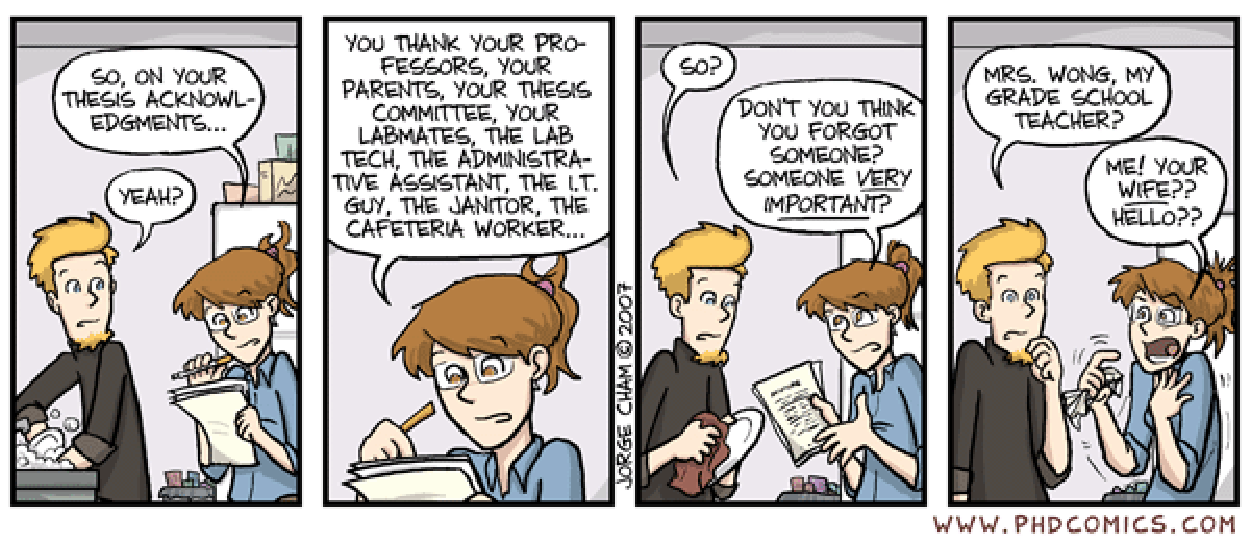
\includegraphics[width=.9\linewidth]{./graphics/phd060607s}\footnote{Source: 
%\url{http://phdcomics.com/}, no.~870 and 871}

%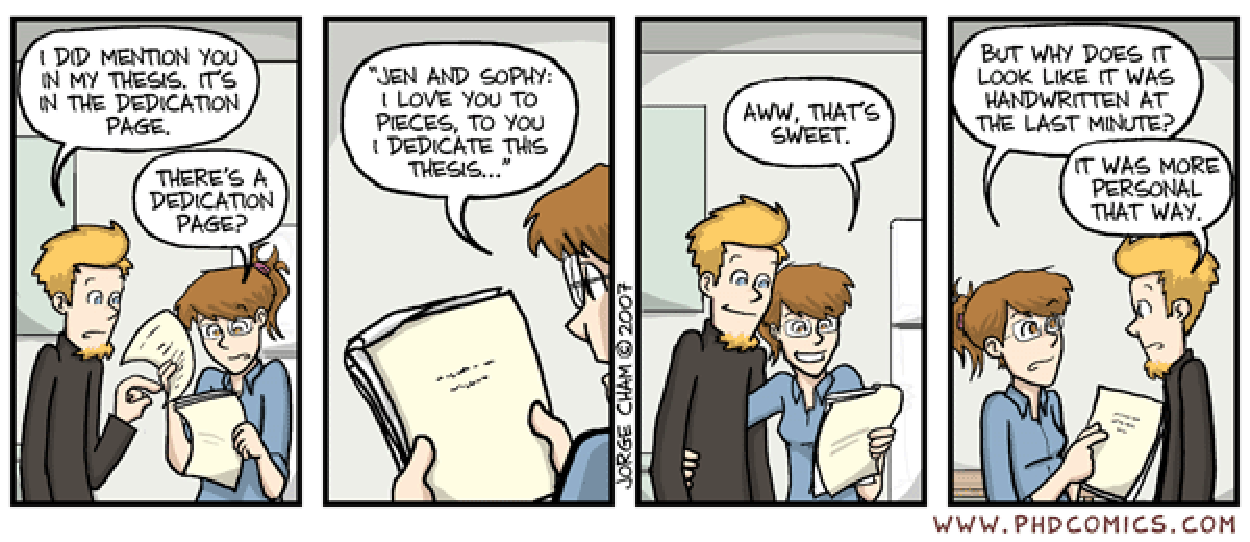
\includegraphics[width=.9\linewidth]{./graphics/phd060807s}
%\end{center}



%You should probably use \texttt{\textbackslash chapter*} for
%acknowledgements at the beginning of a thesis and
%\texttt{\textbackslash chapter} for the end.

%%% Local Variables: 
%%% mode: latex
%%% TeX-master: "../mythesis"
%%% End: 


%------------------------------------------------------------------------------
% CV needed when you submit your PhD thesis
% \definecolor{lightgray}{gray}{0.8}
\newcolumntype{L}{>{\raggedleft}p{0.15\textwidth}}
\newcolumntype{R}{p{0.8\textwidth}}
\newcommand\VRule{\color{lightgray}\vrule width 0.5pt}

\thispagestyle{empty}
\section*{Curriculum Vitae}

\subsection*{Personal Details}

\begin{tabular}{L!{\VRule}R}
Name & YiFan Wang 王一帆 \\
Date of Birth & 27.05.1990 \\
Email & yfwang@thp.uni-koeln.de \\
Family status & Single
\end{tabular}

\subsection*{Education}

\begin{tabular}{L!{\VRule}R}
%2006--2009 & Abitur, ABC Secondary School, Hamburg, Germany\\
2009--2014 & BSc in Physics, Peking University, Beijing, China.\\
2014--2017 &  MSc in Physics, Rheinische Friedrich-Wilhelms-Universität, Bonn, 
Germany. \\
\end{tabular}

\subsection*{Professional Experience}

\begin{tabular}{L!{\VRule}R}
2013 & DESY Summer Student, Zeuthen, Germany. \\
2006 & Master thesis at Universit\"at zu K\"oln, Cologne, Germany. \\
\end{tabular}

\subsection*{Languages}
\begin{tabular}{L!{\VRule}R}
Mandarin & Mother tongue
English & C1 \\
German & B2 \\
\end{tabular}


\end{document}

%%% Local Variables:
%%% mode: latex
%%% TeX-master: t
%%% End:
